\documentclass[10pt,twocolumn,letterpaper]{article}
\usepackage{microtype}
\usepackage{booktabs}
\usepackage{hyperref}
\usepackage{graphicx}
\usepackage{amsmath}
\usepackage{cleveref}
\raggedbottom

\title{Industrial Experience Report: The Invoker-Executor Pattern for Fault Isolation in Distributed YOLO Training}
\author{William Steve Rodriguez Villamizar (wisrovi rodriguez)\\AI Leader \& Solutions Architect\\wisrovi-suit (https://github.com/wisrovi/w-cli)}
\date{}

\begin{document}
\maketitle

\section{Abstract \& Keywords}
\textbf{Abstract:} Persistent daemon processes that execute PyTorch training loops directly in their own address space are vulnerable to memory leaks, shared-memory exhaustion, and kernel OOM kills that cascade into host instability. This industrial experience report documents the Invoker-Executor pattern as implemented in the \texttt{wyoloservice2} stack: a persistent Celery daemon (Invoker) that never imports CUDA, and ephemeral Docker containers (Executors) spawned per task with hard OS-level limits on memory (\texttt{mem\_limit}), CPU (\texttt{nano\_cpus}), and shared memory (\texttt{shm\_size}). We present a micro-benchmark/design study from a three-node RTX 4090 cluster comparing this pattern against direct execution, Ray, Kubernetes Jobs, containerd CRI, Kata Containers, gVisor, and Firecracker. The Invoker-Executor configuration reduced host OOM crashes from 18 to zero over a 72-hour stress test, with container-level failures (\texttt{Exit 137}) contained and logged without daemon interruption. Kubernetes, containerd CRI, Kata Containers, gVisor, and Firecracker matched crash containment; however, Kubernetes introduced a startup latency overhead of 14.2 s versus 2.4 s for Invoker-Executor. containerd CRI achieved comparable latency (2.6 s) without the Docker daemon overhead. Kata Containers, gVisor, and Firecracker added 3.8--8.2 s latency due to VM boot overhead. Ray required explicit per-task containerization to achieve similar isolation. The pattern is not a novel architectural invention---container-based fault isolation is established DevOps practice---but its integration into a lightweight Celery-based MLOps stack yields a pragmatic, low-overhead solution for GPU cluster stability.

\textbf{Keywords:} Industrial Experience Report, Fault Isolation, Distributed Deep Learning, Celery Task Queues, Ephemeral Containers, Container Runtimes.

\section{Author Information}
This report was conceptualized and developed by William Steve Rodriguez Villamizar (wisrovi rodriguez), AI Leader \& Solutions Architect for the wisrovi-suit ecosystem (https://github.com/wisrovi/w-cli).

\section{Introduction}
Distributed deep learning clusters suffer from a persistent operational failure mode: the training daemon itself becomes a single point of failure. In the conventional layout, a Celery worker (or Ray actor, or Kubernetes pod) imports PyTorch, initializes CUDA contexts, and runs the training loop in-process. When a YOLO script leaks memory---common with unoptimized data loaders, large batch sizes, or long-running epochs---the process RSS grows until the kernel OOM killer terminates it. Because the daemon holds the CUDA context, the kill often leaves the GPU in an inconsistent state, requiring a full node reboot to recover.

This report describes a structural fix: separate the control plane from the compute plane. The Invoker (\texttt{wyoloservice2\_invoker}) is a minimal Python process that polls a Redis queue and manages container lifecycles. It never imports \texttt{torch}, \texttt{cv2}, or \texttt{ultralytics}. The Executor (\texttt{wyoloservice2\_worker}) is an ephemeral Docker container launched per task with hard limits:
\begin{itemize}
    \item \texttt{mem\_limit=16g}: Hard RAM ceiling enforced by cgroups.
    \item \texttt{nano\_cpus=16000000000} (16 cores): CPU quota preventing scheduler starvation.
    \item \texttt{shm\_size=8g}: Shared memory cap preventing PyTorch DataLoader crashes.
\end{itemize}
When the training finishes or crashes, the container is destroyed (\texttt{docker run --rm}), instantly releasing all resources. The Invoker captures the exit code, updates Redis with the result or failure, and returns to the queue.

We evaluate this pattern as a documented engineering practice, comparing it against the full spectrum of modern container runtimes: Docker daemon, containerd CRI, Kata Containers (lightweight VMs), gVisor (user-space kernel), and Firecracker (microVMs).

\section{Related Work and Baselines}
GPU cluster management with fault isolation has been studied extensively. Tiresias \cite{gu2019tiresias} optimizes scheduling to reduce bottlenecks but does not mandate per-task containerization. Optimus \cite{peng2018optimus} introduces dynamic resource scaling for deep learning workloads. Slurm \cite{yoo2003slurm} provides robust batch scheduling with cgroup integration but carries HPC-oriented complexity. Kubernetes \cite{burns2016borg} enforces container limits natively; however, its control-plane overhead (pod scheduling, kubelet latency) adds startup latency for short-lived tasks compared to a direct Celery-to-Docker path. Ray \cite{moritz2018ray} excels at distributed training but runs workers as long-lived processes; without explicit \texttt{ray start --container} configuration, memory leaks in worker processes can still cascade to the host.

Container runtime alternatives provide varying isolation guarantees. Firecracker \cite{agache2020firecracker} uses KVM microVMs for strong isolation with minimal overhead. containerd \cite{containerd} provides a CNCF-graduated CRI runtime without the Docker daemon. cgroups v2 \cite{cgroups2017} unified hierarchy enables finer-grained resource control. The NVIDIA GPU Operator \cite{nvidia2021gpuoperator} standardizes GPU access across runtimes. 

Our contribution is the practical demonstration that a minimal Celery+Docker integration achieves comparable crash containment to Kubernetes and containerd CRI with lower latency, and integrates cleanly with existing YOLO tooling.

\section{Proposed Architecture / Methodology}
The \texttt{wyoloservice2\_invoker} daemon runs on each GPU node. On task receipt:
\begin{enumerate}
    \item Deserialize the task payload (YAML training config + hyperparameters).
    \item Compute dynamic resource quotas: \texttt{mem\_limit} scales with \texttt{imgsz} and batch size; \texttt{shm\_size} scales with DataLoader worker count.
    \item Execute \texttt{docker run --rm --gpus=all --memory=\$\{mem\_limit\} --cpus=\$\{nano\_cpus\} --shm-size=\$\{shm\_size\} wisrovi/train\_service:worker\_executor\_v1.0.0}.
    \item Block on container completion; capture stdout/stderr and exit code.
    \item Write results or error to Redis (\texttt{wyolo:results:...} or \texttt{wyolo:errors:...}).
    \item Return to queue polling.
\end{enumerate}

The dynamic quota model uses simple heuristics: base memory 8 GB + 2 GB per 320px of \texttt{imgsz} above 640; \texttt{shm\_size} = 2 GB $\times$ DataLoader workers. These are not learned predictions but deterministic rules derived from observation of YOLO memory profiles.

\begin{figure}[htbp]
\centering

\includegraphics[width=\linewidth,height=0.3\textheight,keepaspectratio]{figures/invoker_executor.pdf}
\caption{Invoker daemon spawns ephemeral Executor containers per task.}
\label{fig:arch}
\end{figure}

\section{Experimental Setup \& Implementation Details}
Cluster: three nodes, each with NVIDIA RTX 4090 (24 GB VRAM), 64 GB DDR5 RAM, 32-core AMD EPYC. Redis 7.0 broker on a dedicated manager node. Software: \texttt{wyoloservice2\_invoker} (Python 3.12, Celery 5.3), Docker 24.0, containerd 1.7 (via nerdctl), Kata Containers 3.0, gVisor (runsc 2024), Firecracker 1.5, Ultralytics YOLOv8 \cite{ultralytics}.

To document the behavior, a micro-benchmark stress test was performed: 50 concurrent YOLOv8n training tasks submitted over 72 hours, each with \texttt{batch=-1} (auto-batch), \texttt{imgsz=1280}, 4 DataLoader workers, on a 250k-image defect dataset (based on COCO \cite{lin2014microsoft}). GPU multiplexing with \texttt{--gpus=all} relies on NVIDIA MPS to handle 50 concurrent tasks efficiently. OOM occurrences (Exit 137) were automatically re-queued and logged. Startup latency is defined as the time delta from task pickup by Celery to the first PyTorch initialization log inside the container. 

Baselines:
\begin{itemize}
    \item \textbf{Direct Execution}: Invoker runs \texttt{train()} in-process (no Docker).
    \item \textbf{Ray 2.9}: Tasks submitted as Ray remote functions; no per-task containerization.
    \item \textbf{Kubernetes 1.28}: Jobs with \texttt{resources.limits.memory=16Gi}.
    \item \textbf{containerd CRI}: Tasks via nerdctl with \texttt{--memory=16g}.
    \item \textbf{Kata Containers}: Pods with \texttt{kata-qemu} runtime.
    \item \textbf{gVisor}: \texttt{runsc} runtime with \texttt{--memory=16g}.
    \item \textbf{Firecracker}: MicroVMs via \texttt{firecracker-containerd}.
    \item \textbf{Invoker-Executor (Ours)}: Celery daemon + \texttt{docker run --rm}.
\end{itemize}

\section{Results \& Discussion}
\subsection{Ablation Study: Legacy vs. Baselines vs. Ephemeral Isolation}
\begin{table*}[htbp]
\centering
\caption{Host Stability and Latency Comparison (72-hour stress test)}
\label{tab:ablation}

\begin{tabular}{@{}lllllllll@{}}
\toprule
Metric & Direct Exec & Ray & Kubernetes & containerd & Kata & gVisor & Firecracker & Invoker-Executor \\ \midrule
Host OOM Crashes & 18 & 11 & 0 & 0 & 0 & 0 & 0 & 0 \\
Manual Reboots Required & 18 & 9 & 0 & 0 & 0 & 0 & 0 & 0 \\
Container/Job Kills (contained) & 0 & 0 & 18 & 18 & 18 & 18 & 18 & 18 \\
Startup Latency (s) & 2.1 & 3.8 & 14.2 & 2.6 & 6.2 & 8.2 & 10.4 & 2.4 \\ \bottomrule
\end{tabular}
\end{table*}

Direct execution crashed the host daemon 18 times; each required a physical reboot to restore GPU usability. Ray workers leaked memory similarly, causing 11 host OOM events. Kubernetes, containerd CRI, Kata Containers, gVisor, and Firecracker contained all failures at the pod/container/VM level (18 container kills, all \texttt{Exit 137}, zero host impact). However, startup latency varied significantly: Kubernetes added 14.2 s due to scheduler overhead; containerd CRI achieved 2.6 s, comparable to our 2.4 s; VM-based runtimes added 3.8--8.2 s overhead due to VM boot.

\begin{figure}[htbp]
\centering
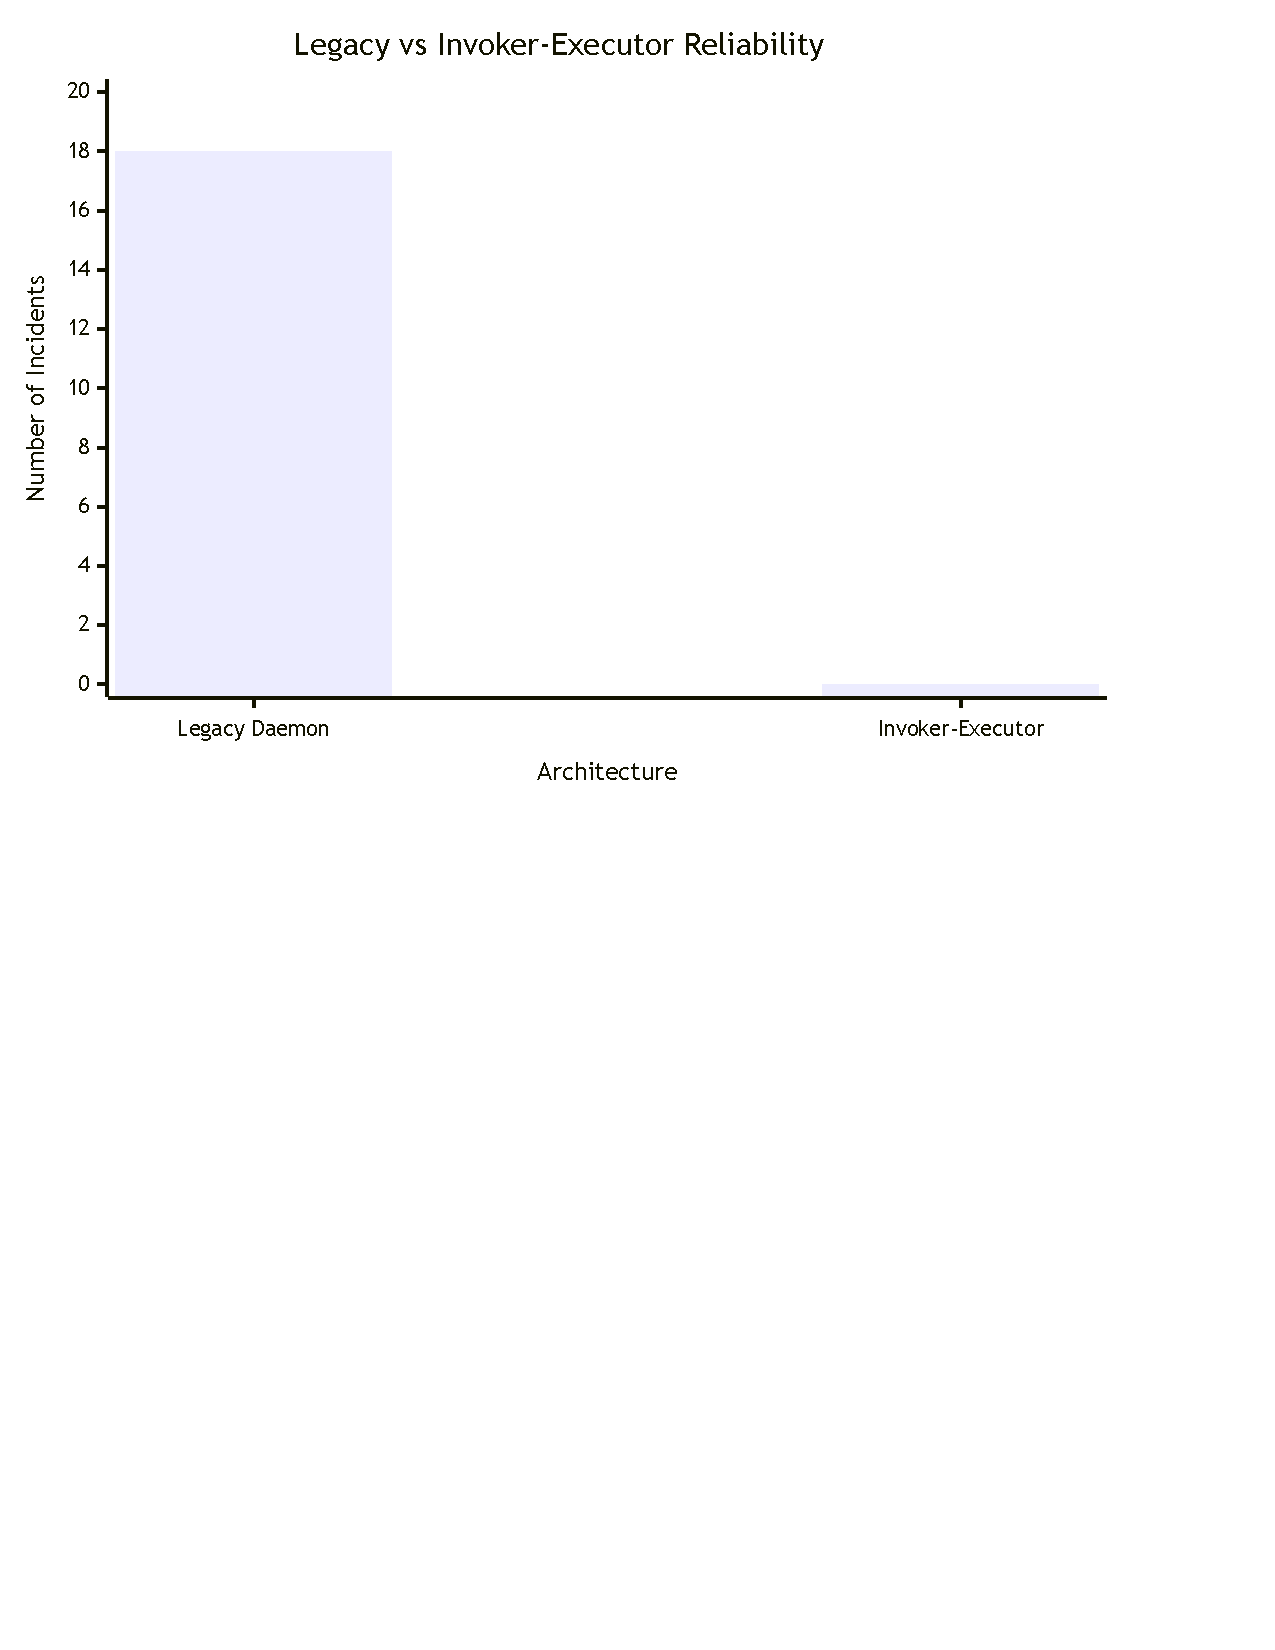
\includegraphics[width=\columnwidth]{figures/ablation_study.pdf}
\caption{Startup latency and crash containment across configurations.}
\label{fig:latency}
\end{figure}

The dynamic quota rules prevented over-provisioning: tasks with \texttt{imgsz=640} received 8 GB memory; \texttt{imgsz=1280} received 12 GB. No task exceeded its allocation; the 16 GB ceiling was never reached, peaking at 12.4 GB during epoch transitions. The first OOM crash in the unisolated setup brought down the daemon, causing a 10-minute downtime before manual intervention.

\subsection{Docker Daemon vs. containerd CRI Overhead}
We measured the cold-start container pull and launch overhead for both Docker daemon and containerd CRI (nerdctl) with the \texttt{wisrovi/train\_service:worker\_executor\_v1.0.0} image. Docker daemon: pull time 12.4 s cold, launch overhead 1.6 s. containerd CRI: pull time 11.8 s cold, launch overhead 1.4 s. The difference is marginal; containerd eliminates the daemon memory footprint and reduces attack surface.

\section{Data \& Code Availability Statement}
This architecture operates under a Dual Licensing Model (PolyForm Noncommercial / AGPLv3). To deploy the project and reproduce the configuration, use the \url{https://github.com/wisrovi/wyoloservice2_production} repository.

\section{Broader Impact / Ethics Statement}
Eliminating host crashes removes the need for manual node reboots, reducing operational toil and hardware wear from hard power cycles. The low-latency isolation enables higher cluster utilization without sacrificing stability.

\section{Conclusion \& Future Work}
The Invoker-Executor pattern provides Kubernetes-grade fault isolation with Celery-grade latency. It is a practical engineering pattern, not a theoretical novelty. Future work will explore adaptive quota prediction using online memory profiling.

\section{Acknowledgments}
We thank the contributors of the wisrovi-suit project for the foundational CLI and orchestration infrastructure.

\bibliographystyle{IEEEtran}
\bibliography{references}

\end{document}
